%Part of/Parte di https://github.com/f-dinucci/appuntiMeccanicaFluidi/
%License/Licenza Creative Commons Attribution-ShareAlike 4.0 International (CC BY-SA 4.0) - attribution/attribuzione Francesco Di Nucci
%See also/Vedere anche https://creativecommons.org/licenses/by-sa/4.0/ and/e https://creativecommons.org/licenses/by-sa/4.0/legalcode
%
\section{Manometri}
%Subsection
\subsection{Manometri}
Per manometro si intende un qualsiasi strumento per la misura della pressione di un fluido, negli esempi che seguono se ne vedrà un sottoinsieme ristretto basato sulla misurazione dell'altezza di una colonna di fluido.
La scelta del liquido impiegato nel manometro è legata al campo di pressione da misurare: si usano ad esempio mercurio, acqua ed alcool, ma è teoricamente possibile usare anche gas.
%Subsubsection
\subsubsection{Manometro semplice a colonna}
Il manometro semplice a colonna di liquido è costituito da un tubo ad U, parzialmente riempito con un liquido.
Uno dei bracci del barometro è collegato ad un serbatoio ad una certa pressione (da misurare), l'altro all'atmosfera.
Misura pertanto la pressione relativa tra il serbatoio e l'atmosfera.
	\begin{figure}[ht]
		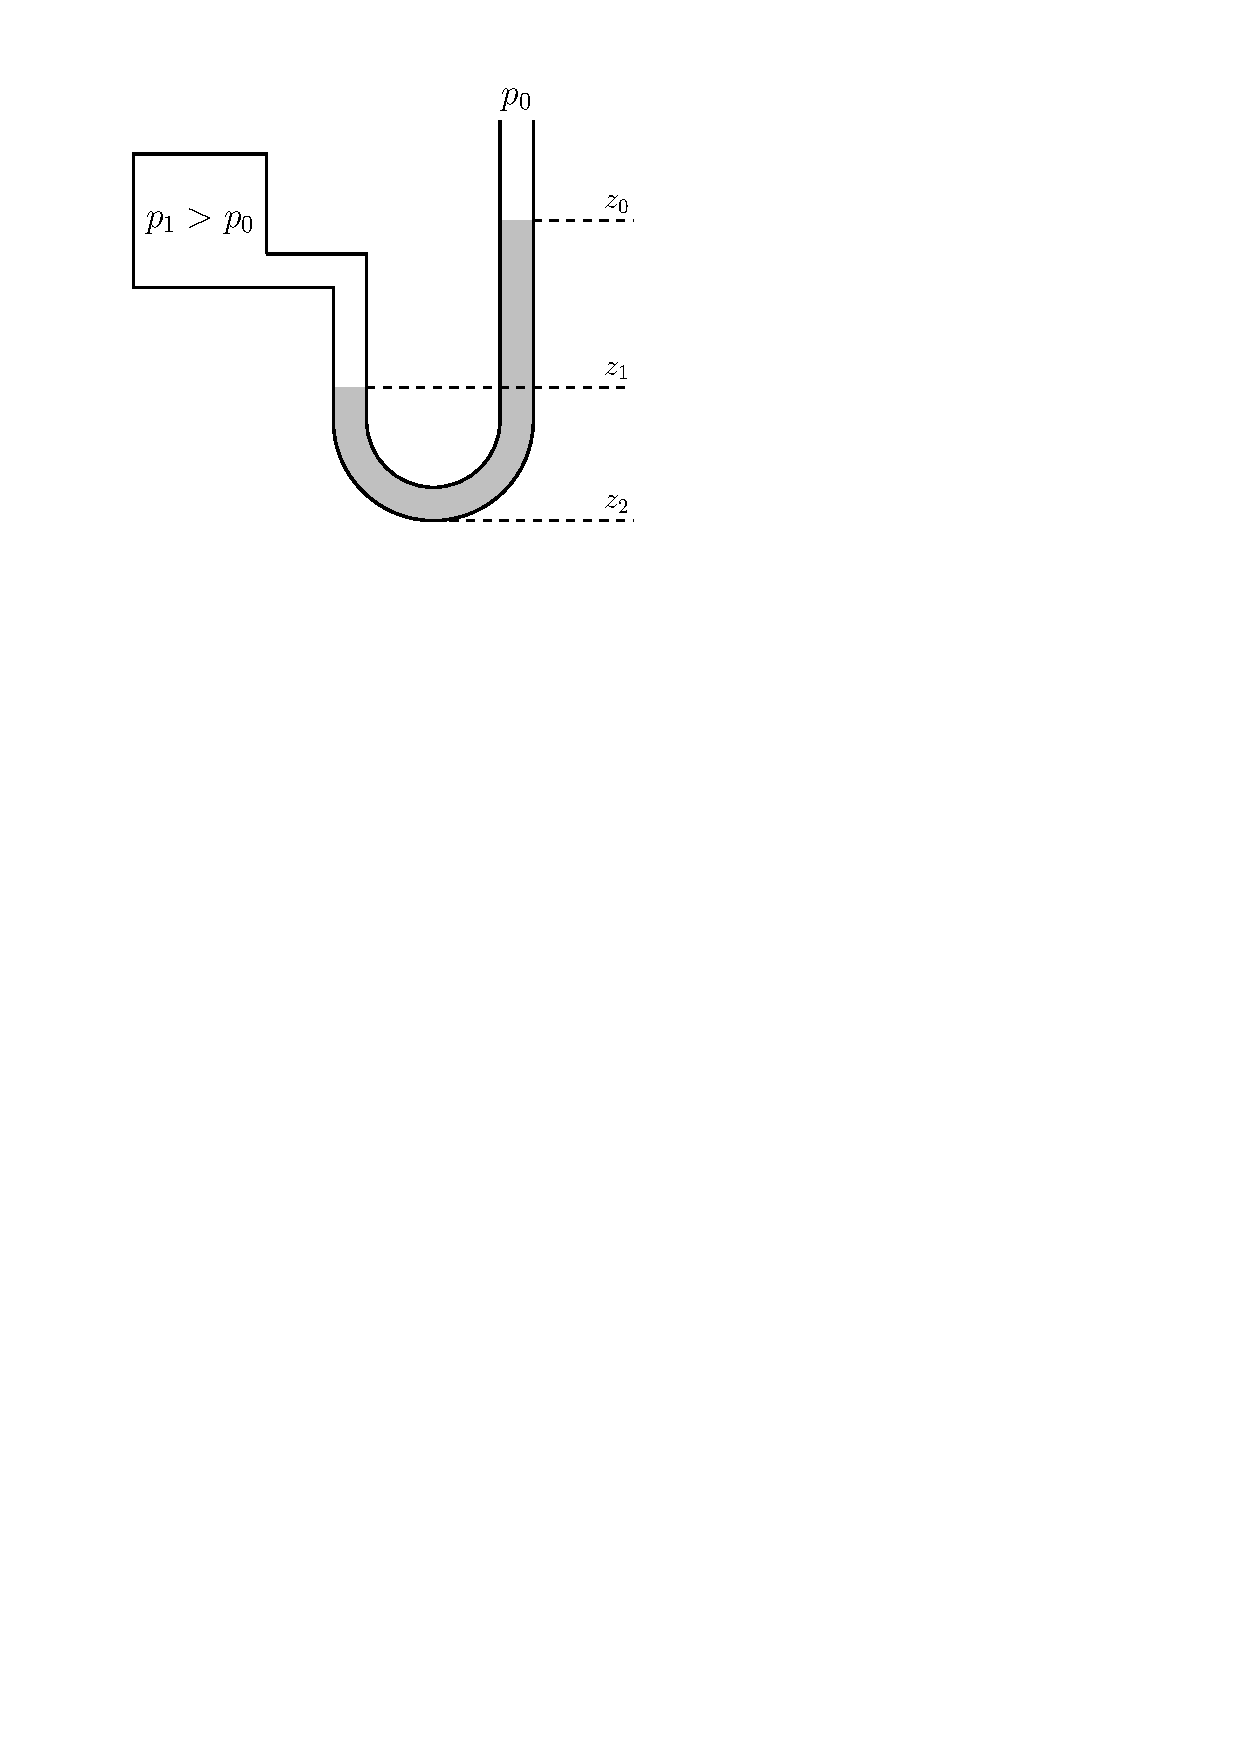
\includegraphics[scale=0.80]{./2.3 Manometri/2.3-1}
		\centering
		\caption{Manometro a colonna, $p_1 > p_0$}
	\end{figure}

	\begin{figure}[ht]
		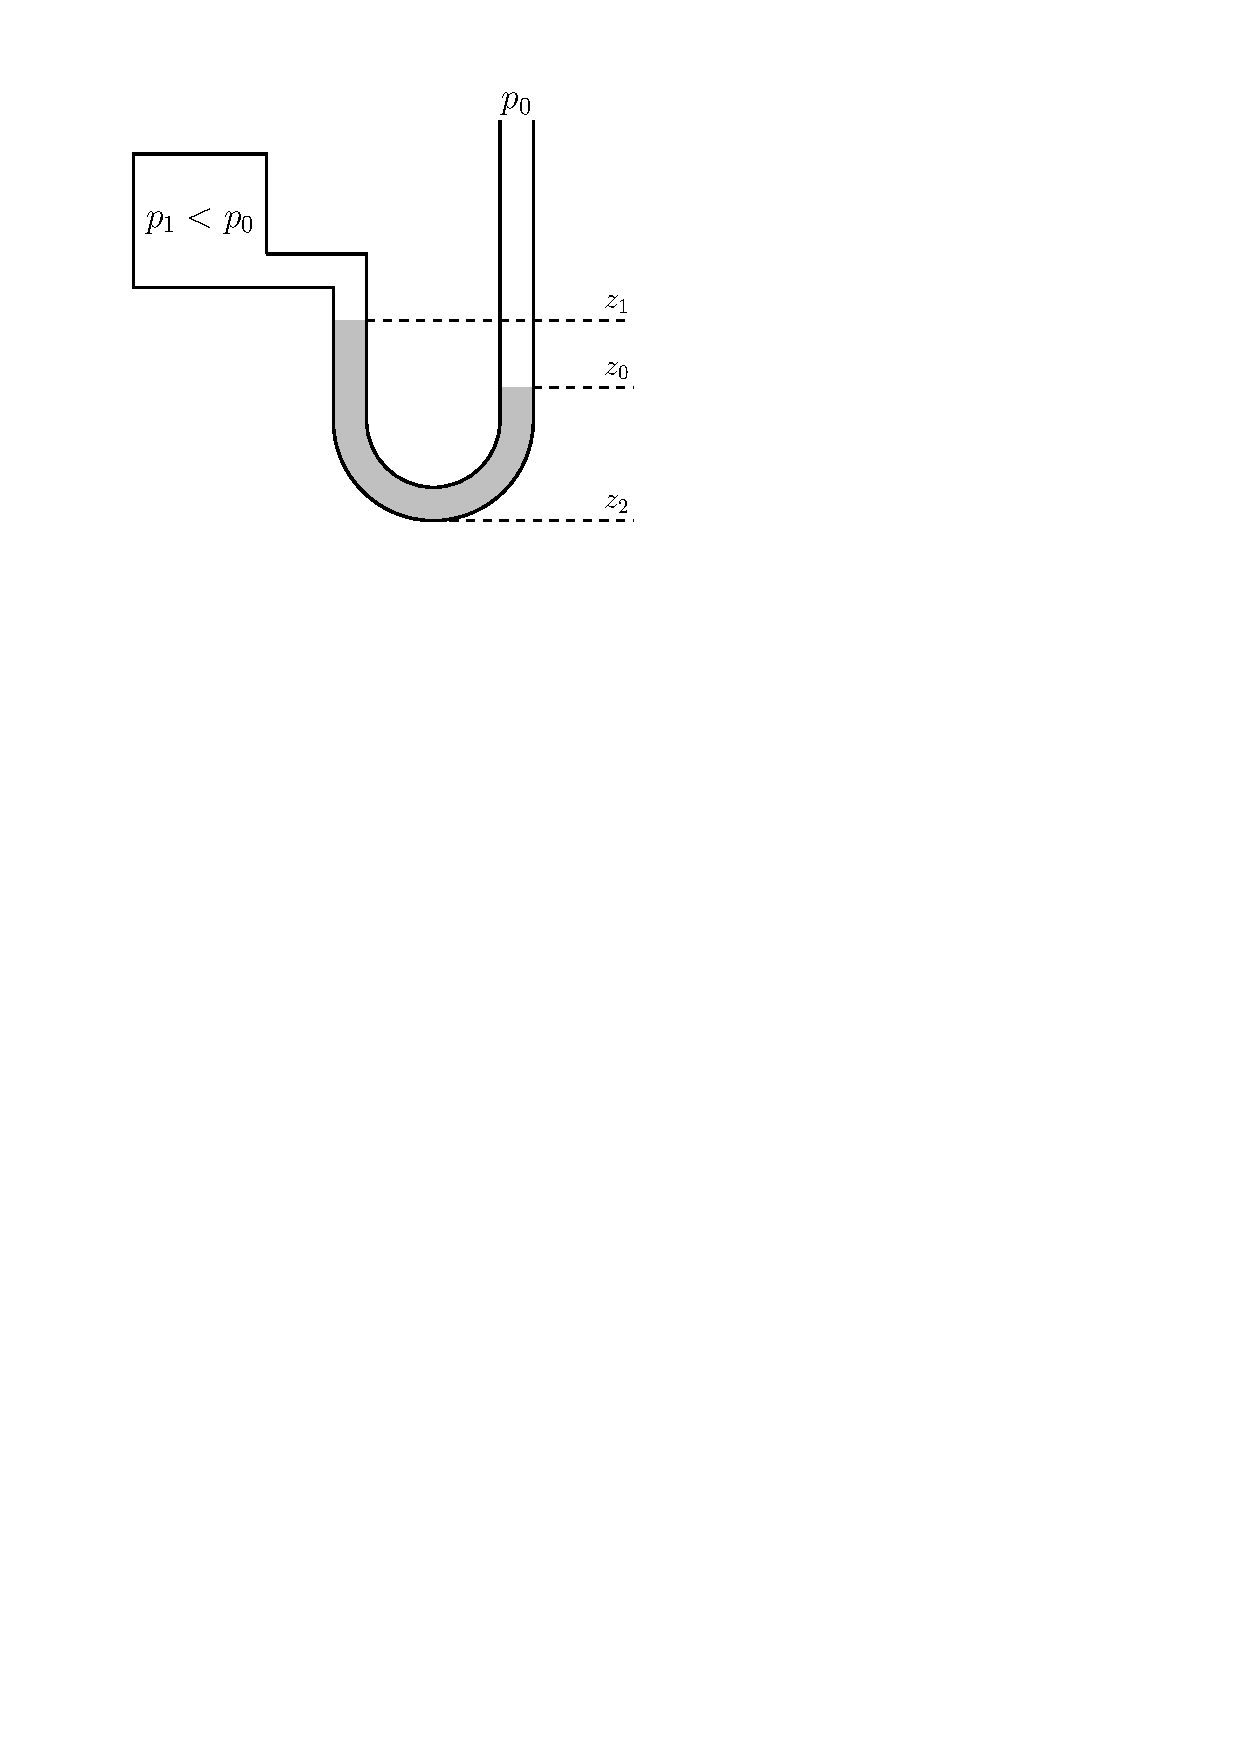
\includegraphics[scale=0.80]{./2.3 Manometri/2.3-2}
		\centering
		\caption{Manometro a colonna, $p_1 < p_0$}
	\end{figure}
	
Definito $h$ il dislivello del liquido tra i due bracci del manometro (vedere in seguito), si ha che, dalle equazioni nei due bracci:
	\begin{equation*}
		\begin{gathered}
			\left\{ 
			\begin{gathered}
				p_2 = p_1 + \rho g (z_1 - z_2) \\ 
				p_2 = p_0 + \rho g (z_0 - z_2) 
			\end{gathered} 
			\right. \\
			\text{Eguagliando}\\
			 p_1 + \rho g (z_1 - z_2) = p_0 + \rho g (z_0 - z_2)\\
			 \text{da cui}\\
			 p_1 = p_0 + \rho g (z_0 - z_1)\\
			 \text{infine, per evidenziare se $p$ sia maggiore o minore di $p_0$}\\
			 \left\{
			 \begin{gathered}
				p_1 > p_0 \rightarrow h = z_0 - z_1 \rightarrow p_1 = p_0 + \rho g h\\ 
				p_1 < p_0 \rightarrow h = z_1 - z_0 \rightarrow p_1 = p_0 - \rho g h
			\end{gathered} 
			\right. \\
		\end{gathered}	
	\end{equation*}
	

%Subsubsection
\subsubsection{Manometro inclinato}
Un manometro inclinato funziona in maniera analoga ad uno a colonna, solo che uno dei due bracci è inclinato ed ha una sezione molto più piccola rispetto all'altro.
Questo comporta che il livello del liquido nel braccio di sezione maggiore sia pressoché costante, con la variazione di quota dovuta alla pressione che si verifica praticamente solo nel braccio inclinato.
In questo tipo di barometro non si misura però direttamente la differenza di quota del liquido $H$, ma la lunghezza $L$, correlata geometricamente ad $H$.
Dato che $L > H$, questo permette una maggior precisione di lettura, utile soprattutto nel caso di pressioni piccole.
	\begin{figure}[H]
		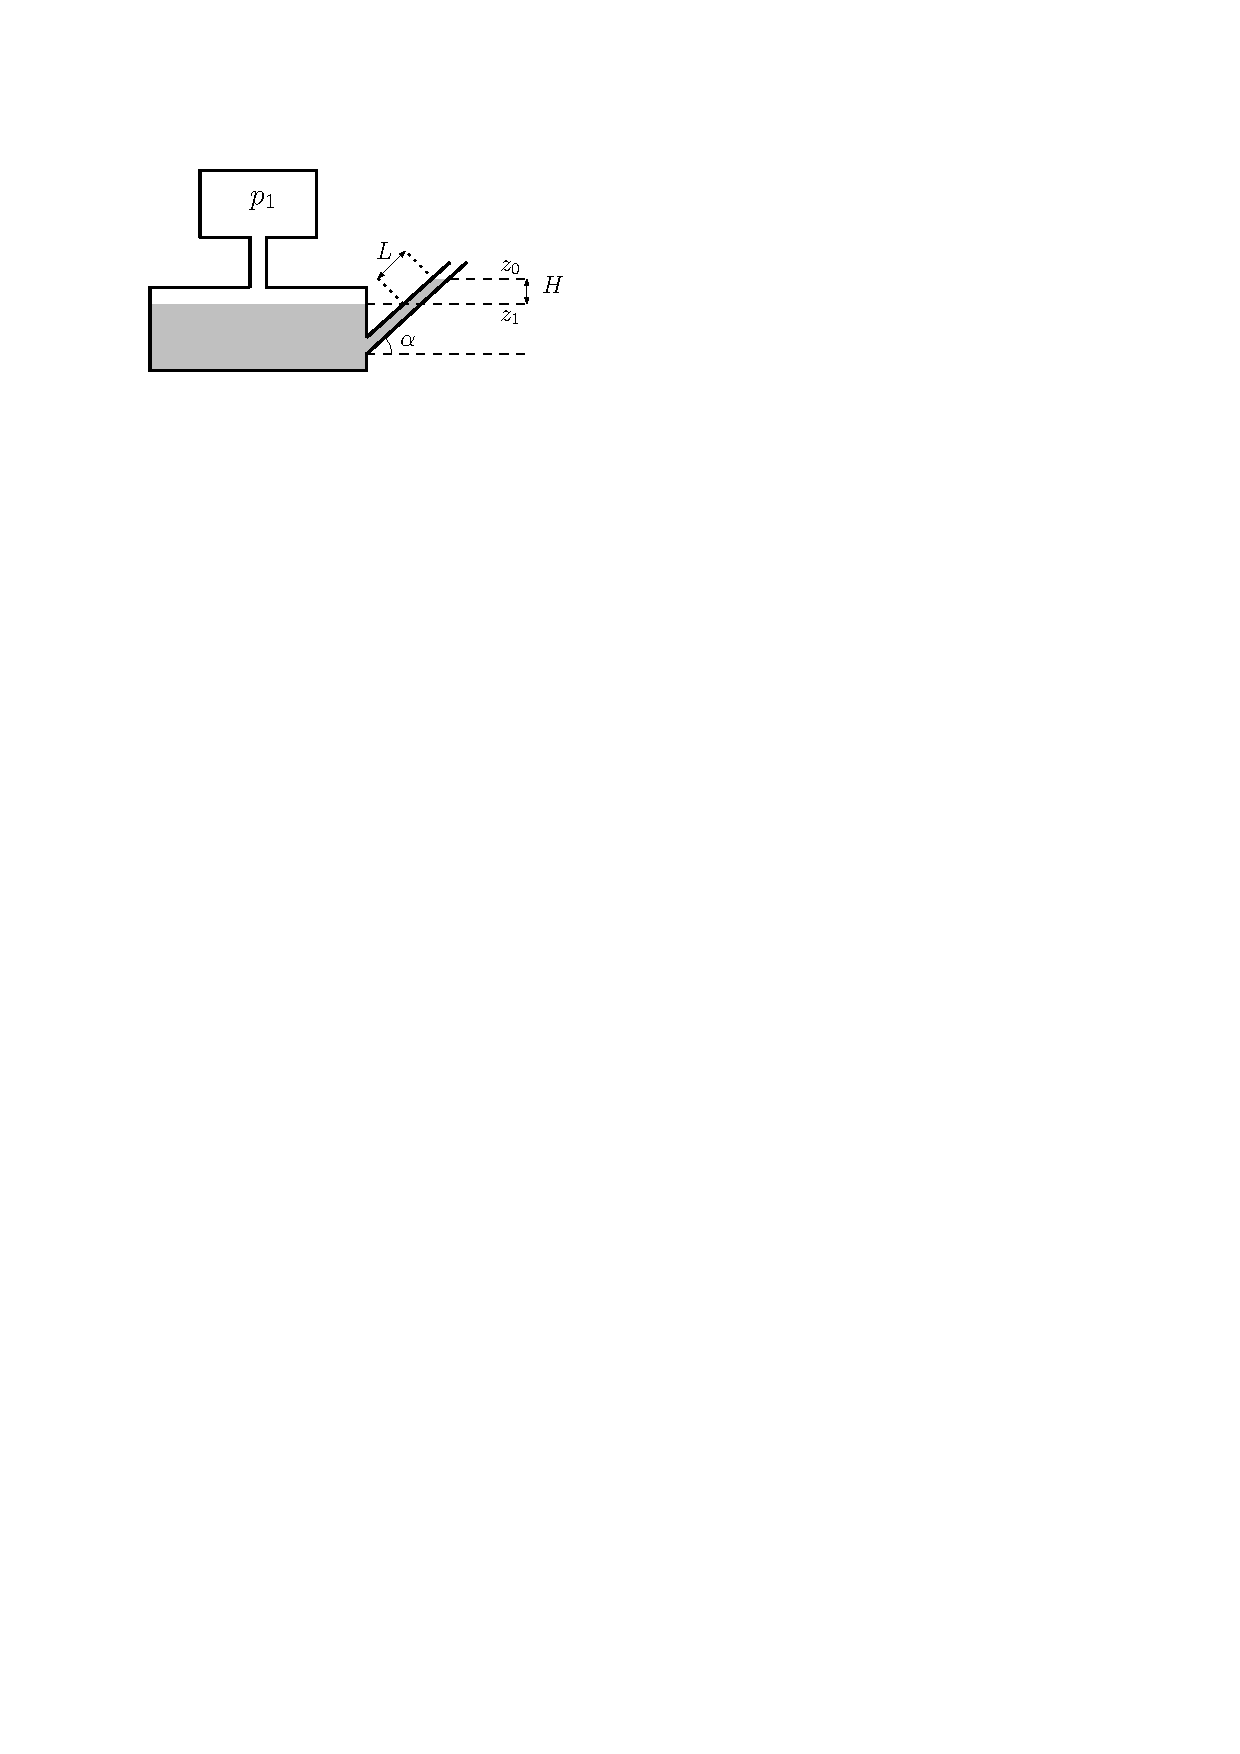
\includegraphics[scale=1.25]{./2.3 Manometri/2.3-3}
		\centering
		\caption{Manometro inclinato, $p_1 > p_0$}
	\end{figure}
Da un punto di vista matematico si ha che:
	\begin{equation*}
		p_1 = p_0 + \rho g H = p_0 + \rho g L \sin{\alpha}
	\end{equation*}
%Subsubsection
\subsubsection{Barometro e pressione atmosferica}
Un barometro è un particolare manometro utilizzato per la misurazione della pressione atmosferica.
Può essere un manometro a colonna con uno dei bracci chiuso e l'altro di sezione molto maggiore oppure da un tubo chiuso ad un estremo, riempito di liquido, poi tappato e posto verticalmente in una bacinella piena dello stesso liquido, ove viene stappato.
Dove il tubo è chiuso si avrà una pressione pari a quella di vapore del liquido utilizzato nel barometro, e dato che si utilizzano liquidi con una bassa pressione di vapore, questa può essere considerata trascurabile.
Si ha quindi che:
	\begin{equation*}
		\begin{gathered}
			\cancel{p_1} = p_0 + \rho g (z_0 - z_1) \\
			p_0 = \rho g (z_1 - z_0)
		\end{gathered}
	\end{equation*}
	
	\begin{figure}[ht]
		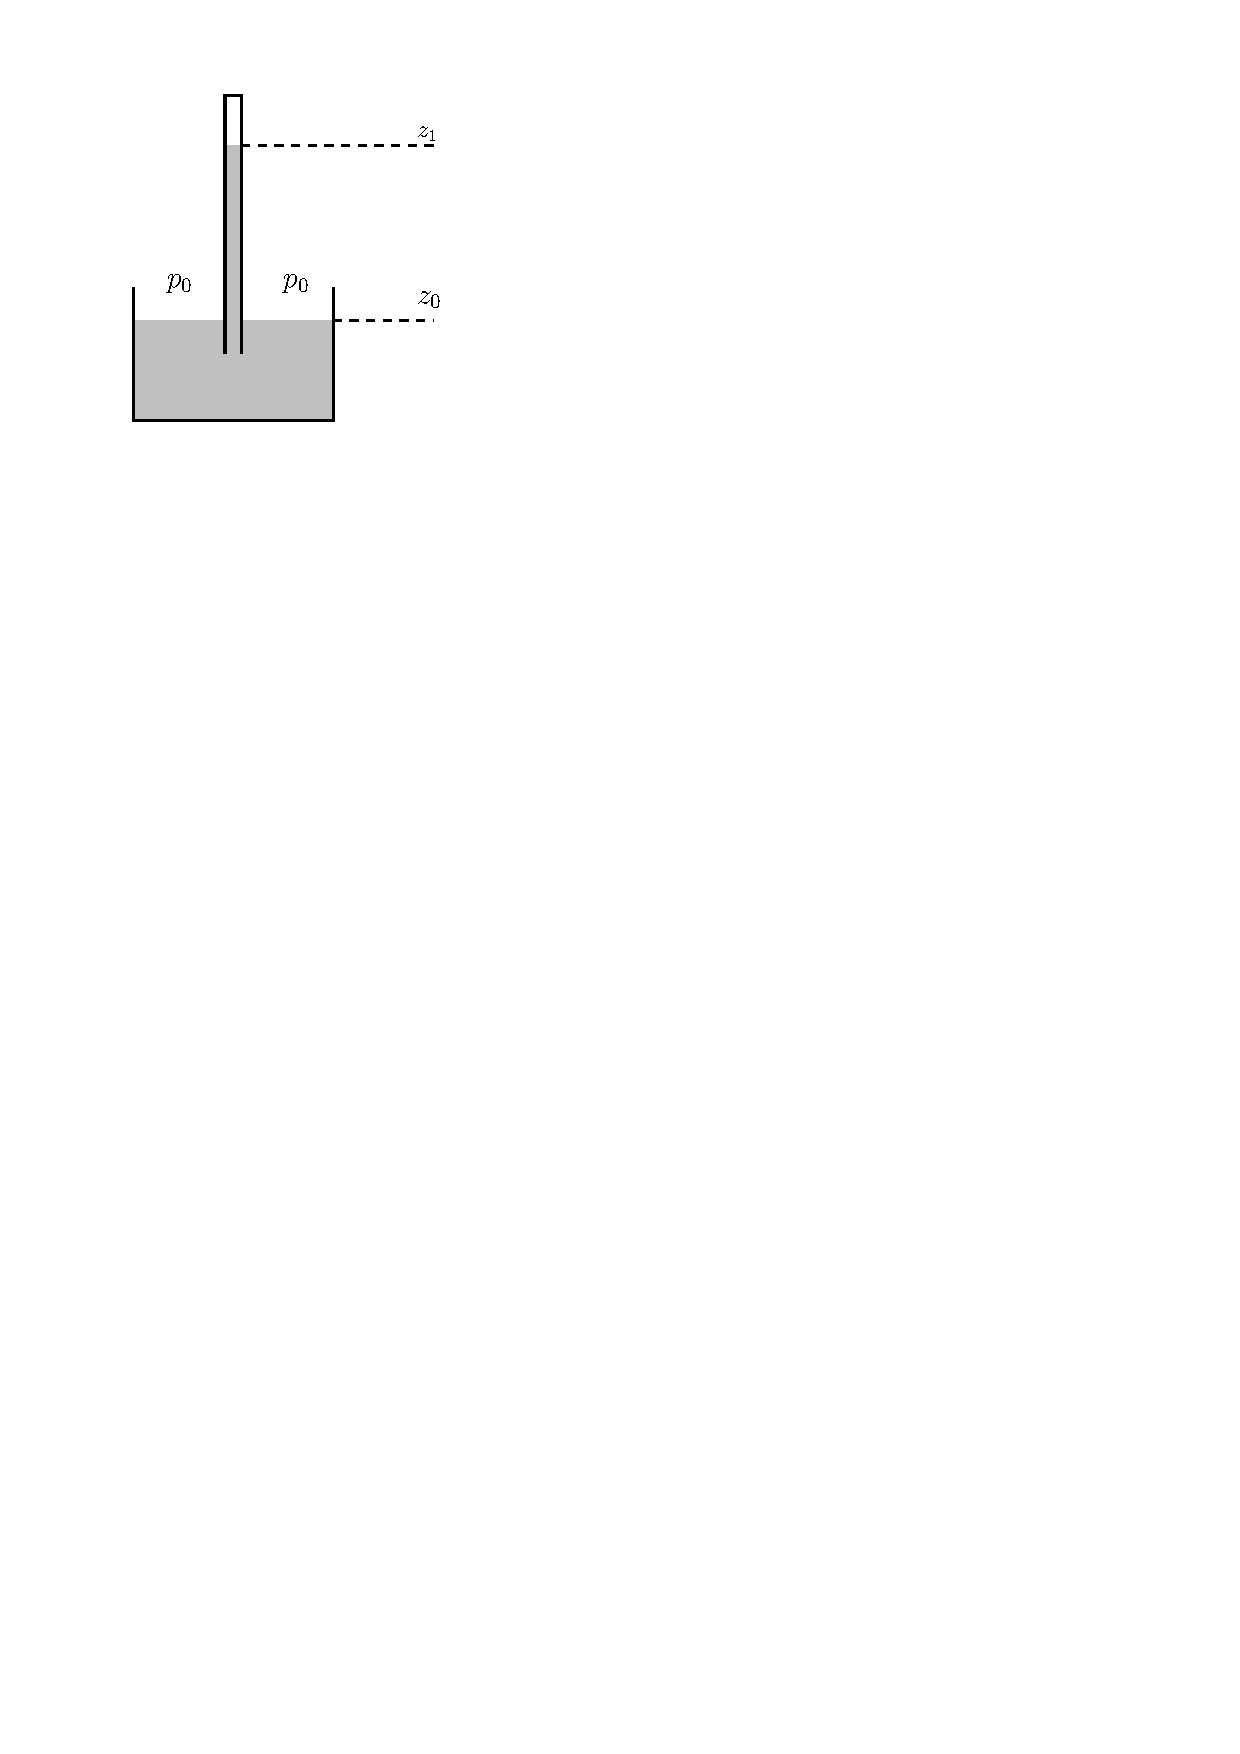
\includegraphics[scale=0.80]{./2.3 Manometri/2.3-4}
		\centering
		\caption{Barometro}
	\end{figure}
	
Da questo si introduce come unità di misura il millimetro di mercurio (mmHg), anche noto come Torricelli (torr)\footnote{in onore dell'italiano Evangelista Torricelli, primo a misurare sperimentalmente la pressione atmosferica}, che equivale alla pressione esercitata da una colonna di mercurio alta \SI{1}{\milli \meter}.
Dato che per eguagliare la pressione atmosferica\footnote{che è il peso per unità di area dell'atmosfera sulla superficie terrestre} in media al livello del mare occorre una colonna di mercurio alta \SI{760}{\milli \meter}, si ha che 760 mmHg = 1 atm.
A confronto, se al posto del mercurio si utilizzasse acqua, sarebbe necessaria una colonna di fluidi alta \SI{10.73}{\meter}.
La misurazione della pressione atmosferica è importante per le conseguenze della sua variazione, legate alle condizioni meteorologiche o a variazioni di quota.
%Subsubsection
\subsubsection{Manometro multifluido}
Un manometro multifluido è un manometro nei cui bracci sono utilizzati più fluidi diversi tra loro e non miscibili tra loro, per rendere la misurazione più agevole od impedire un mescolamento dei fluidi di cui misurare la pressione.
Supponendo di averne uno con tre fluidi distinti, di densità $\rho_1, \rho_2, \rho_3 $ si ha che:
	\begin{equation*}
		\begin{gathered}
			\left\{ 
			\begin{gathered}
				p_2 - p_1 = \rho_1 g (z_1 - z_2)\\ 
				p_2 - p_3  = \rho_2 g (z_2 - z_3)\\
				p_3 - p_0 = \rho_3 g (z_0 - z_3)
			\end{gathered} 
			\right. \\
			\text{da cui}\\
			p_1 = p_0 + \rho_1 g (z_2 - z_1) + \rho_2 g (z_3 - z_2) + \rho_3 g (z_0 - z_3)
		\end{gathered}
	\end{equation*}
Notare che se uno dei fluidi è un gas, la sua densità si può supporre trascurabile rispetto alle altre, è come se trasmettesse la pressione senza variarla.
	\begin{figure}[ht]
		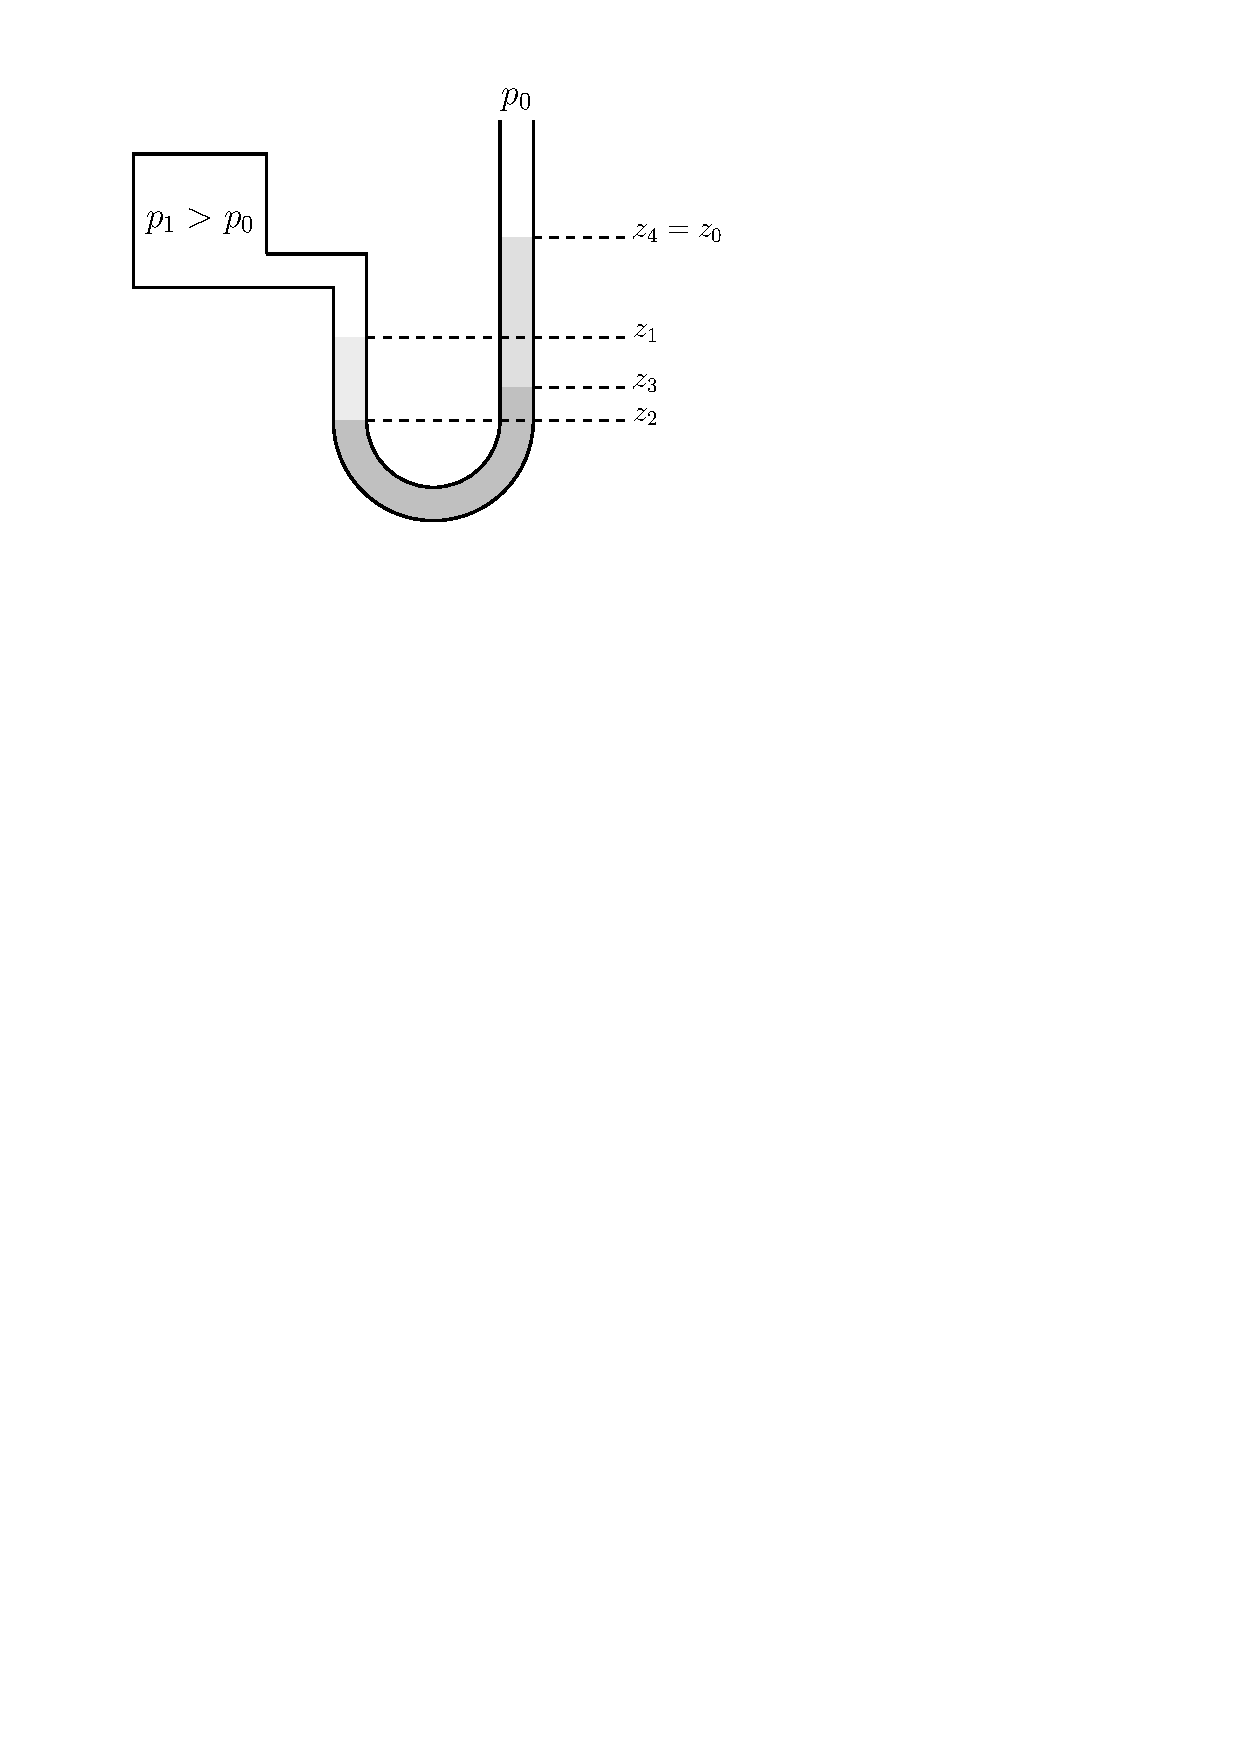
\includegraphics[scale=0.75]{./2.3 Manometri/2.3-5}
		\centering
		\caption{Manometro multifluido con tre fluidi}
	\end{figure}
	
Il ragionamento si può estendere ad \textit{n} fluidi differenti.
Supponendo di numerare progressivamente pressioni, quote e densità a partire da uno, si può generalizzare in:
	\begin{equation*}
		p_1 = p_0 + \sum_{i=i}^{n} \rho_i g (z_{i+1} - z_i)
	\end{equation*}
%Subsubsection
\subsubsection{Manometro differenziale}
Un manometro differenziale non è collegato all'atmosfera, ma si trova ed esempio tra due punti di un condotto a pressioni differenti.
Nella \textit{Figura 2.8} si ha un condotto con un ostacolo che provoca una caduta di pressione, ed è di interesse non tanto la pressione assoluta prima e dopo l'ostacolo, quanto la differenza di pressione tra i due punti.
Quindi al posto di utilizzare due manometri nei due punti distinti per misurare le pressioni e calcolarne poi la differenza, si può utilizzare un manometro differenziale, nel quale si misura la differenza di quota del liquido nei due bracci del manometro.
	\begin{figure}[ht]
		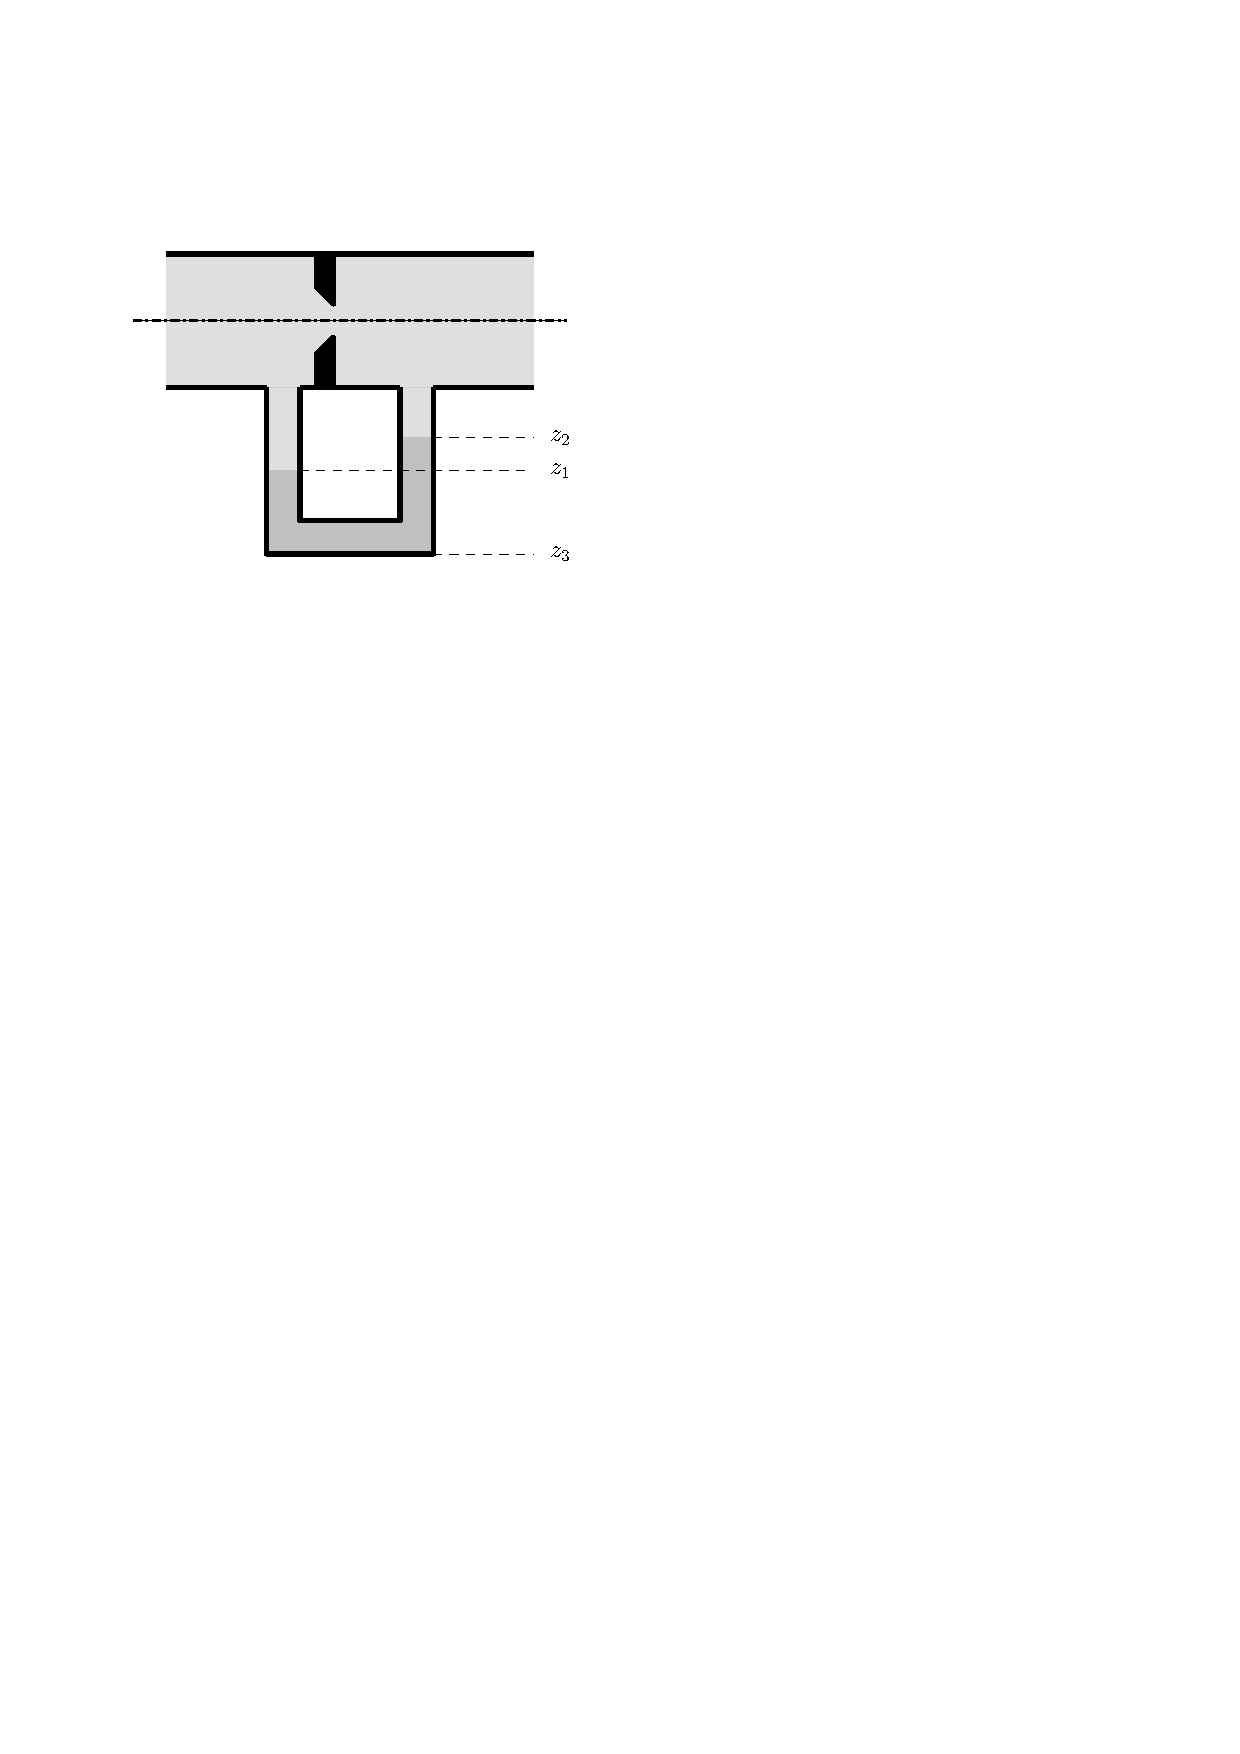
\includegraphics[scale=0.80]{./2.3 Manometri/2.3-6}
		\centering
		\caption{Manometro differenziale}
	\end{figure}
Nei due bracci si ha che la pressione si può esprimere come:
	\begin{equation*}
		\begin{gathered}
			\left\{ 
			\begin{gathered}
				p_3 = p_1 + \rho g (z_1 - z_3)\\ 
				p_3 = p_2 +\rho g (z_2 - z_1)\\
			\end{gathered} 
			\right. \\
			\text{da cui, eguagliando e semplificando}\\
			p_1 - p_2 = \rho g (z_2 - z_1)
		\end{gathered}
	\end{equation*}

\subsection*{Bibliografia 2.3}
\cite[Cap.\ 3.2, 3.3]{CengelCimbala}\\
\cite[Cap.\ 3.2]{PnueliGutfinger}
